%BEGIN: Tatus
\section{A Testbed for Evaluating Human Interaction with Ubiquitous Computing Environments}\label{sec:tatus}

TATUS \cite{o2005testbed} is as a ubiquitous computing simulator aimed at overcoming the challenges of effectively evaluating human interaction with adaptive ubiquitous technologies. These challenges are mainly imposed by the cost and logistics of building and controlling the context in such real-life environments. In other words, TATUS is a simulator supporting research and development of adaptive software controlling ubiquitous computing environments.\\

Figure \ref{fig:tatus_overview} depicts the high-level overview of the simulator. We can identify two main components: the 3D Simulated Ubiquitous Computing Environment and the System Under Test (SUT).\\

\begin{figure}[H]
	\centering
	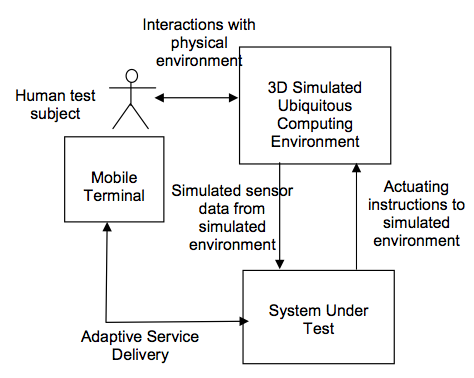
\includegraphics[width=\linewidth]{gfx/Chapter2/tatus_system_overview}
	\caption{High-level simulator overview}
	\label{fig:tatus_overview}
\end{figure}

The 3D simulator was implemented on top of the Half-Life\footnote{\url{http://www.valvesoftware.com}} Game Engine's software development kit (SDK), written in C/C++. Half-Life is a 3D first-person-shooter network game. It is implemented based on client-server architecture with multi-player capabilities (up to 32 players simultaneously). The reason for choosing this game engine was to exploit the 3D graphics engine in order to provide a realistic user experience.\\

The actual simulated environment is created using a map editor from Valve called Hammer (a drawing tool for building maps). This can be used to generate complex and realistic environments as the tool offers a wide range of graphical editing possibilities, as exemplified in Figure \ref{fig:tatus_simulated_meeting_room}. The SDK is then able to load a simulated environment's physical settings from the files generated by the map editor.\\

\begin{figure}[H]
	\centering
	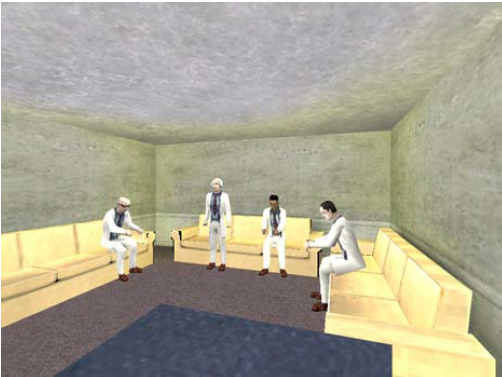
\includegraphics[width=\linewidth]{gfx/Chapter2/tatus_simulated_meeting_room}
	\caption{Simulated meeting room with multiple characters}
	\label{fig:tatus_simulated_meeting_room}
\end{figure}

To simulated sensors and actuators they have exploited a concept called \emph{Triggers} from the SDK. They are used to generate associated events based on a player's movements and location. The state of these triggers together with the agents location at a certain point in time represent the state of the simulated environment. To allow easy access to the data, the simulator exposes an API which offers both querying and modifying capabilities. Queries allow to select certain aspects of the current state based on various parameters, whereas through modifications the SUT can impose changes on the simulated environment.\\

A SUT is written as independent pieces of software. It can even run on a separate machines, while multiple SUTs can connect simultaneously to the same simulator. To allow SUTs to run on separate machines the simulator has embedded networking capabilities and communicates through messages. Outgoing messages carry state information, while incoming messages care instructions to modify the simulated environment. Moreover, to abstract out the network interaction from the SUTs, the simulator provides a Proxy making the communication from the test software's side really easy.\\

\subsection{Conclusions}

One of the main challenges in developing the simulator was that the learning curve of the SDK, in order to extend it, was difficult and time-consuming. But, as a result, they have tried to provide a flexible simulation environment where researchers can easily simulate other environments without the need to modify any SDK level code.\\

The context-awareness is limited to sensors and actuators reacting to the user's position. This is actually not that bad because in the game engine SDK the developer can extract the position of entities, determine proximity of other entities within a given radius and determine the presence of other entities within a field of view. All these data helps to implement simulations for a wide range of sensors.\\

The user control provided by the game engine is pretty advanced allowing the agent to move in any direction, crouch, jump, sit etc. This is a big plus as it adds a good sense of reality to the game.\\

Multiple users can join and experience the same simulated environment at the same time. Not all player have to be human, not-player-characters (controlled by the AI of the engine) can be present as well.\\

Unfortunately the simulator is not open-source so making it unusable for research outside the institution it was developed in.
%END: Tatus